\chapter{Fake Factors}\label{app:fake-factors}
	This appendix contains supplementary material for the fake factor extraction procedure outlined in \ref{sec:bkg-modeling}. Figures \ref{fig:bkg-FF-CR} shows the fake factors for both multijet and W+jets \glspl{CR}. Figure \ref{fig:rQCD} shows the extracted and corrected $\alpha$ values in the \glspl{SR} and \glspl{CR}. Figures \ref{fig:mm:Fits:region3_1} through \ref{fig:mm:Fits:region7_4} show the process of extracting the $\alpha$ values, including the fits.

	\begin{figure}[!thp]
	\begin{center}
	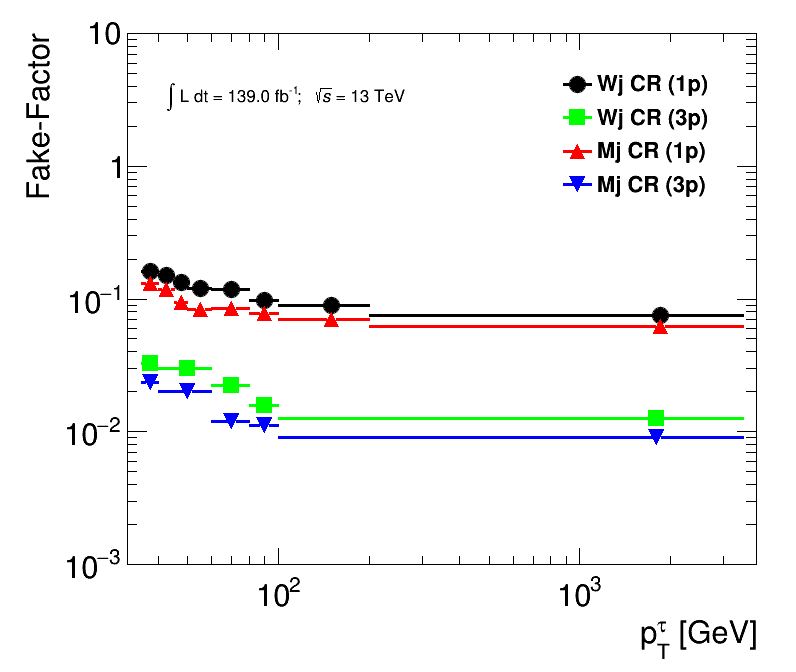
\includegraphics[width=0.45\textwidth]{chapters/chapter6_HPlus/images/FFs/FFs_inclusive_tracks_pT_FFsCR.png}
	\end{center}
	\caption{ Fake factors parameterized as a function of $\pt^{\tau}$ and the number of charged $\tau$ decay products (1-prong and 3-prong) obtained in the multi-jet and W+jets CRs. The errors shown represent the statistical uncertainty. 
	}
	\label{fig:bkg-FF-CR}
	\end{figure}

	\begin{figure}[h!]
	\begin{center}
	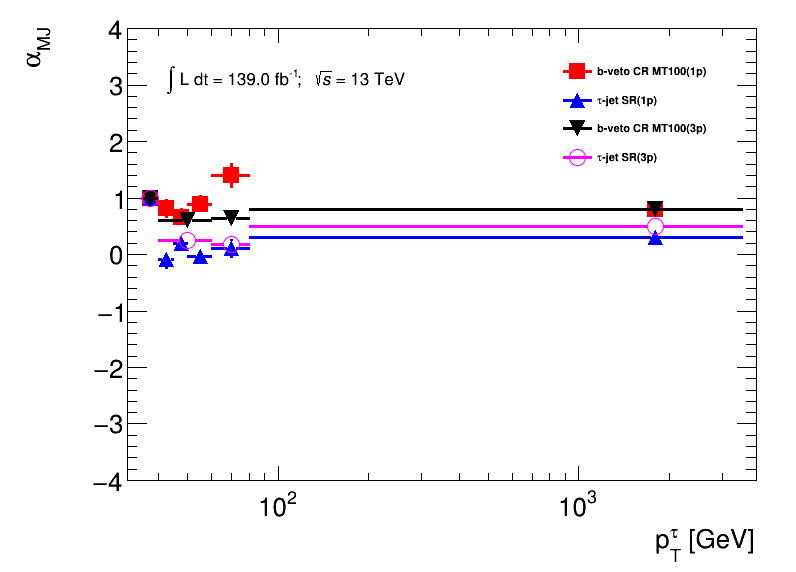
\includegraphics[width=0.45\textwidth]{chapters/chapter6_HPlus/images/FFs/ALPHA_inclusive__taujet.png} \qquad
	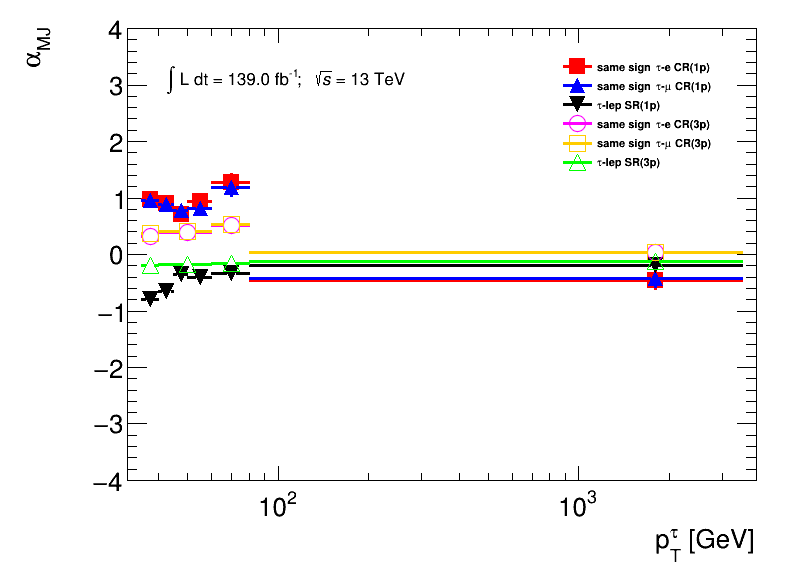
\includegraphics[width=0.45\textwidth]{chapters/chapter6_HPlus/images/FFs/ALPHA_inclusive__taulep.png} 
	\end{center}
	\caption{
	Corrected $\alpha_\mathrm{MJ}$ values for the \tauhad+jets b-veto $\mathrm{m_{T}}>$100 control region, \tauhad+jets signal region, \tauhad+electron(muon) with same-sign control region and the \tauhad+lepton signal region. Error bars represent uncertainties due to $\alpha_\mathrm{MJ}$ fitting using template-fit method. 
	}
	\label{fig:rQCD}
	\end{figure}

	\begin{figure}
	\begin{center}
	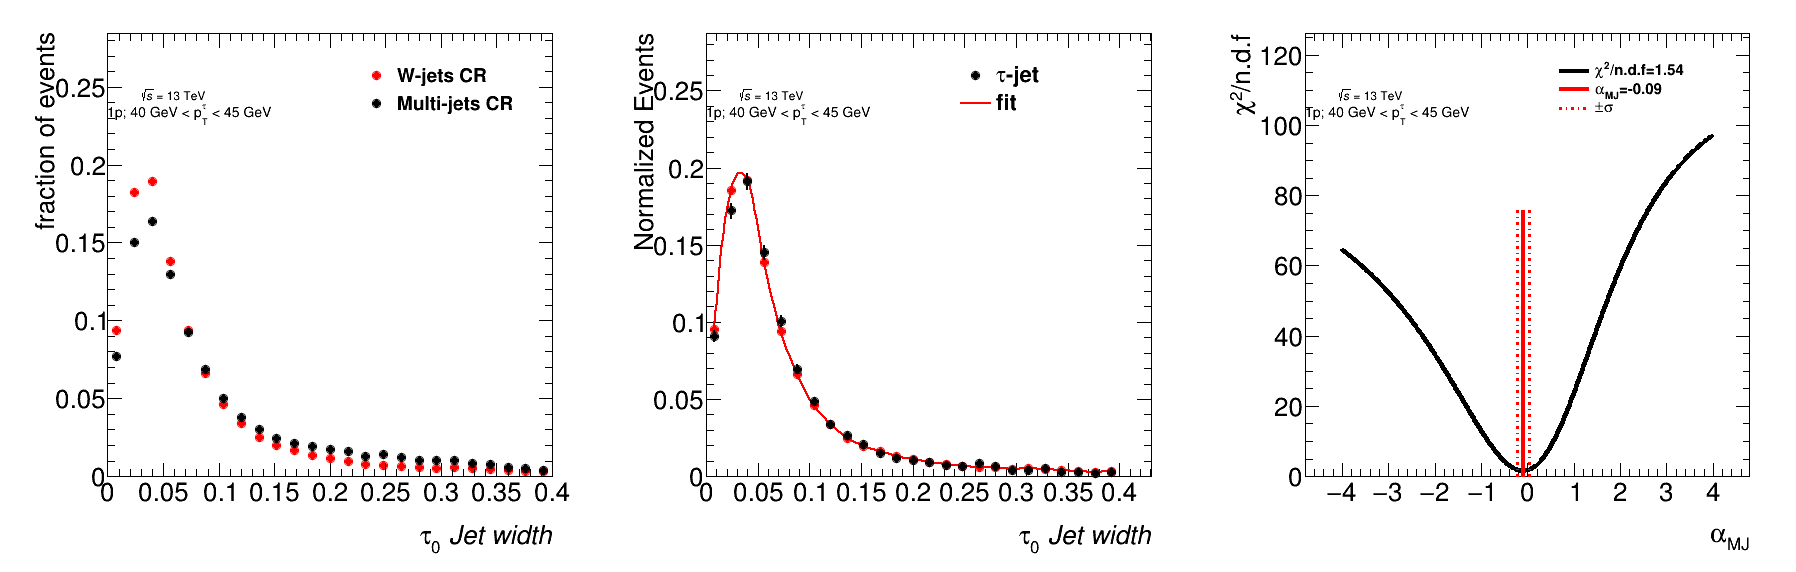
\includegraphics[width=1\textwidth]{chapters/chapter6_HPlus/images/FFs/FFs_FIT_SR_TAUJET_1_40_45.png}
	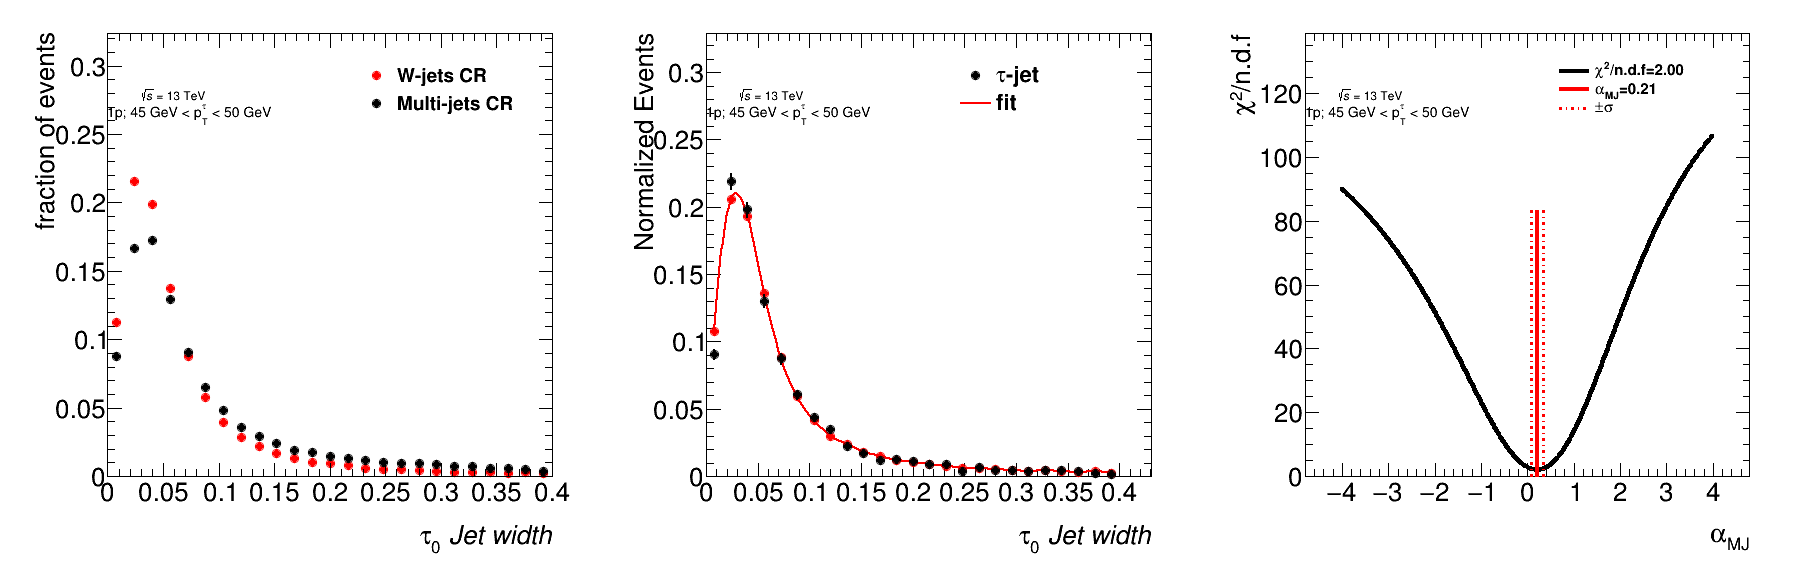
\includegraphics[width=1\textwidth]{chapters/chapter6_HPlus/images/FFs/FFs_FIT_SR_TAUJET_1_45_50.png}
	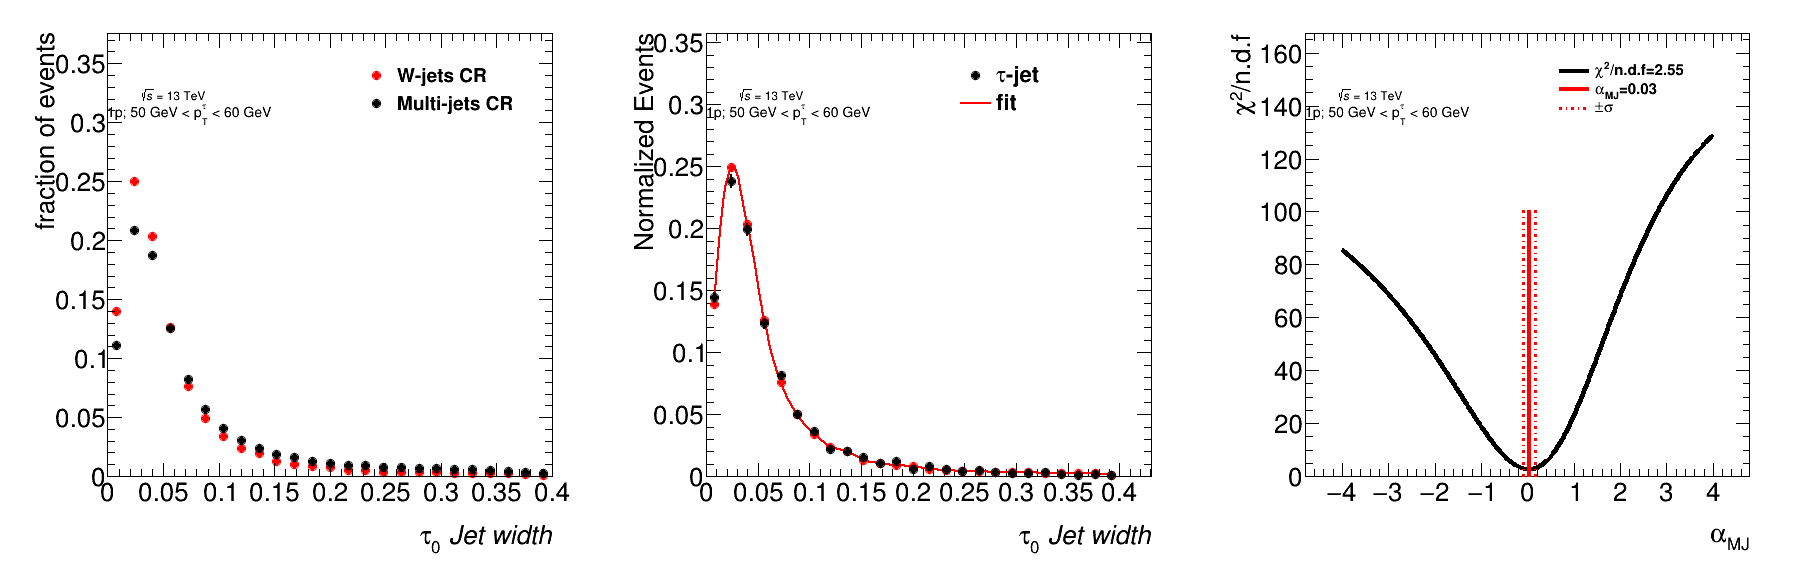
\includegraphics[width=1\textwidth]{chapters/chapter6_HPlus/images/FFs/FFs_FIT_SR_TAUJET_1_50_60.png}

	\end{center}
	\caption{
	Estimation of $\alpha_\mathrm{MJ}$ in the \tauhad+jets signal region for $\pt \leq 60$ GeV 
	1-prong \tauhad candidates. Left: templates of discriminating variables for different \tauhad $\pt$ 
	and n-prong slices. Middle: shape of the discriminating variable obtained in the signal region and fitted 
	shape using the templates measured in the control regions. Right: $\chi^2/\mathrm{ndf}$ of the fit as a 
	function of $\alpha_\mathrm{MJ}$, the error on $\alpha_\mathrm{MJ}$ is defined by the band at 
	$\chi^2_\mathrm{min}/\mathrm{ndf}+\sqrt{\frac{2}{\mathrm{ndf}}}$.
	}

	\label{fig:mm:Fits:region3_1}
	\end{figure}

	\begin{figure}
	\begin{center}
	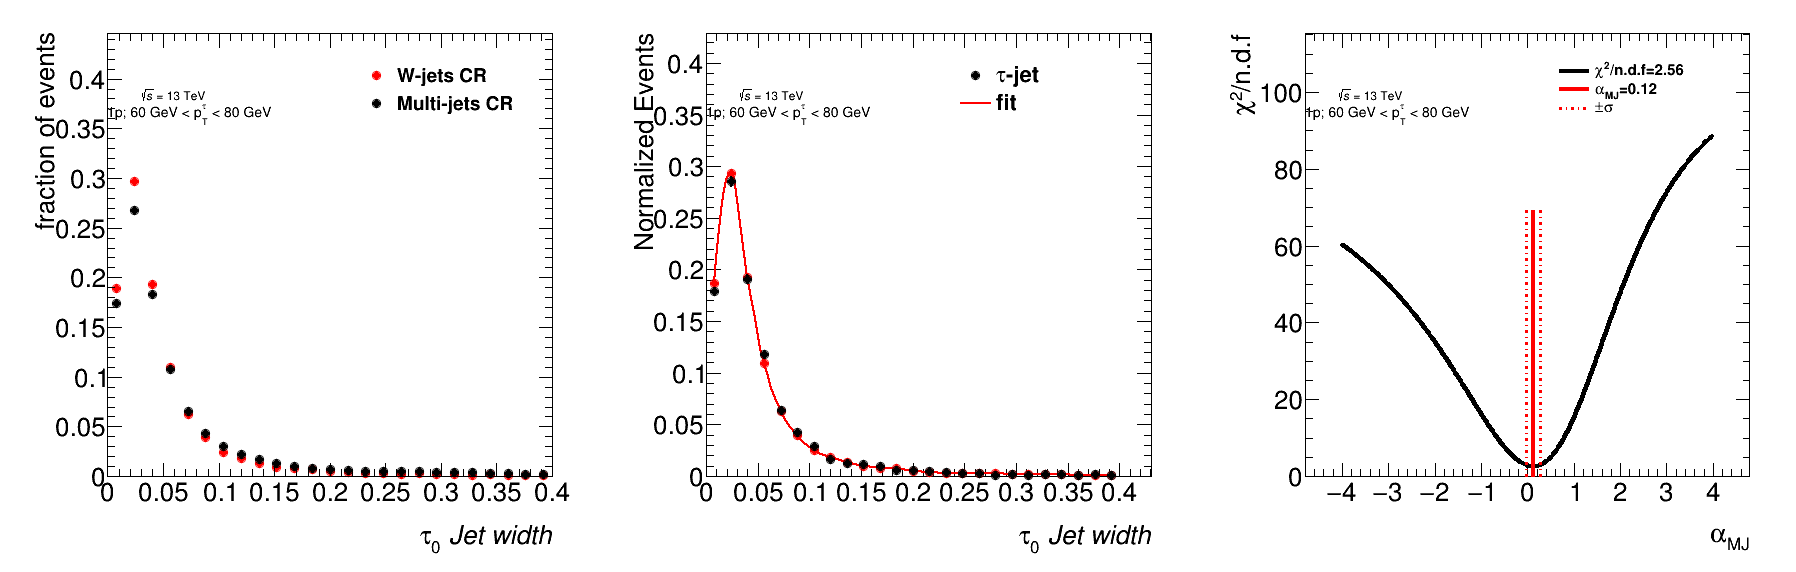
\includegraphics[width=1\textwidth]{chapters/chapter6_HPlus/images/FFs/FFs_FIT_SR_TAUJET_1_60_80.png}
	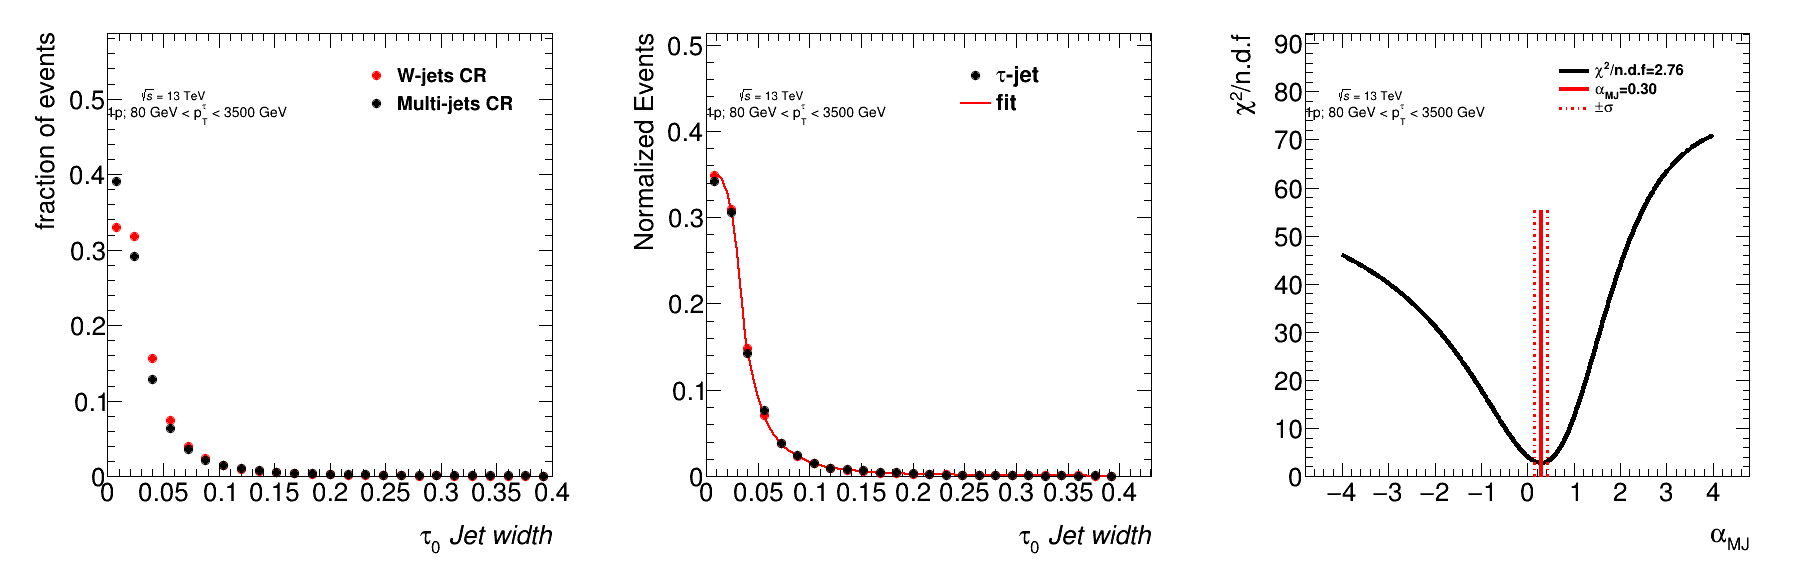
\includegraphics[width=1\textwidth]{chapters/chapter6_HPlus/images/FFs/FFs_FIT_SR_TAUJET_1_80_3500.png}
	\end{center}
	\caption{
	Estimation of $\alpha_\mathrm{MJ}$ in the \tauhad+jets signal region for $\pt \geq 60$ GeV
	1-prong \tauhad\ candidates. Left: templates of discriminating variables for different \tauhad\ $\pt$
	and n-prong slices. Middle: shape of the discriminating variable obtained in the signal region and fitted
	shape using the templates measured in the control regions. Right: $\chi^2/\mathrm{ndf}$ of the fit as a
	function of $\alpha_\mathrm{MJ}$, the error on $\alpha_\mathrm{MJ}$ is defined by the band at
	$\chi^2_\mathrm{min}/\mathrm{ndf}+\sqrt{\frac{2}{\mathrm{ndf}}}$.
	}
	\label{fig:mm:Fits:region3_2}
	\end{figure}

	\begin{figure}
	\begin{center}
	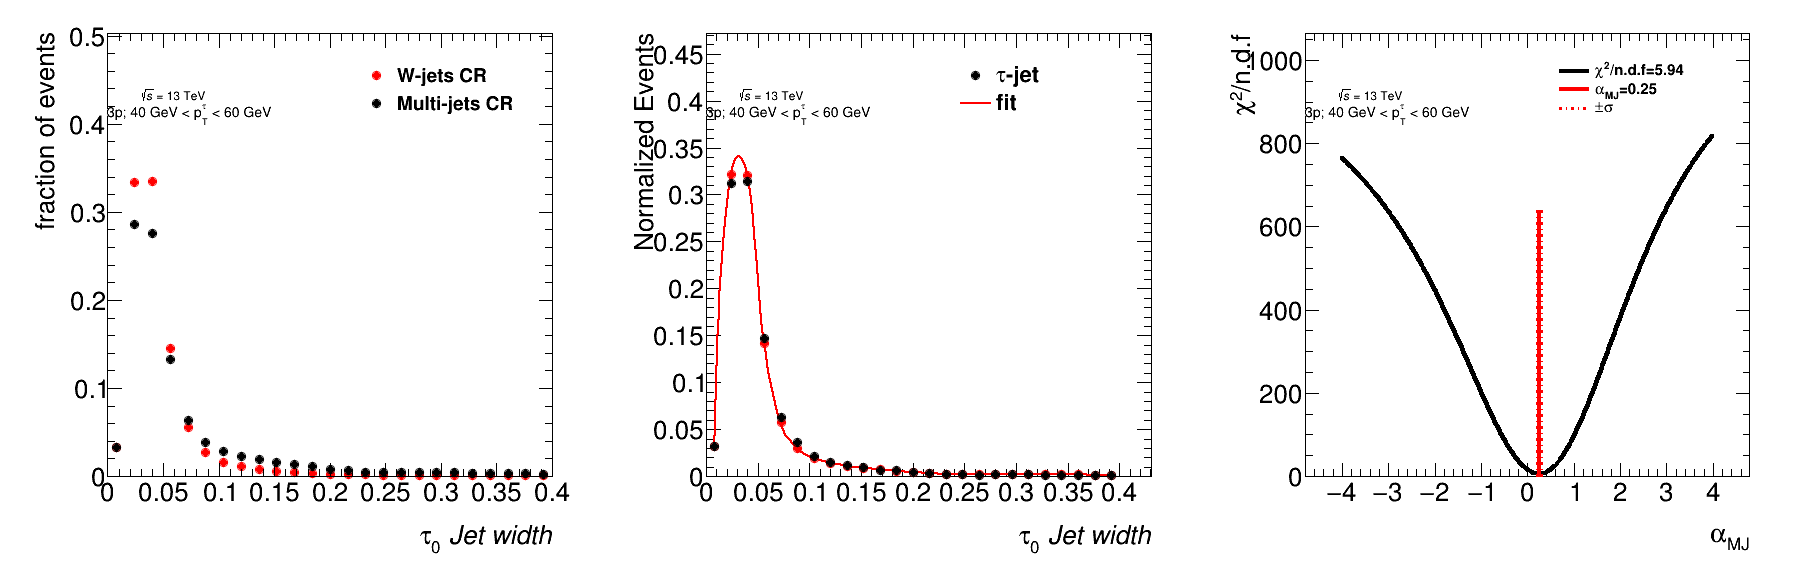
\includegraphics[width=1\textwidth]{chapters/chapter6_HPlus/images/FFs/FFs_FIT_SR_TAUJET_3_40_60.png}
	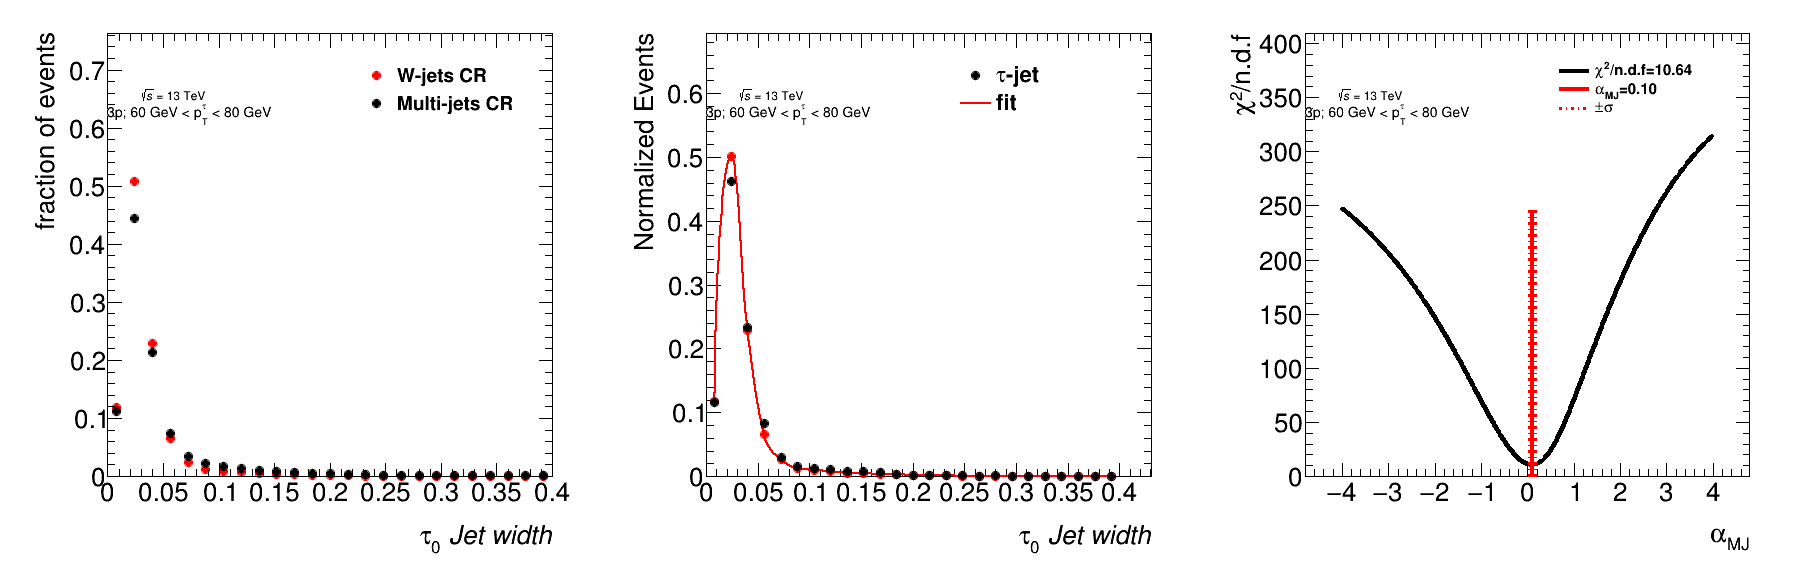
\includegraphics[width=1\textwidth]{chapters/chapter6_HPlus/images/FFs/FFs_FIT_SR_TAUJET_3_60_80.png}
	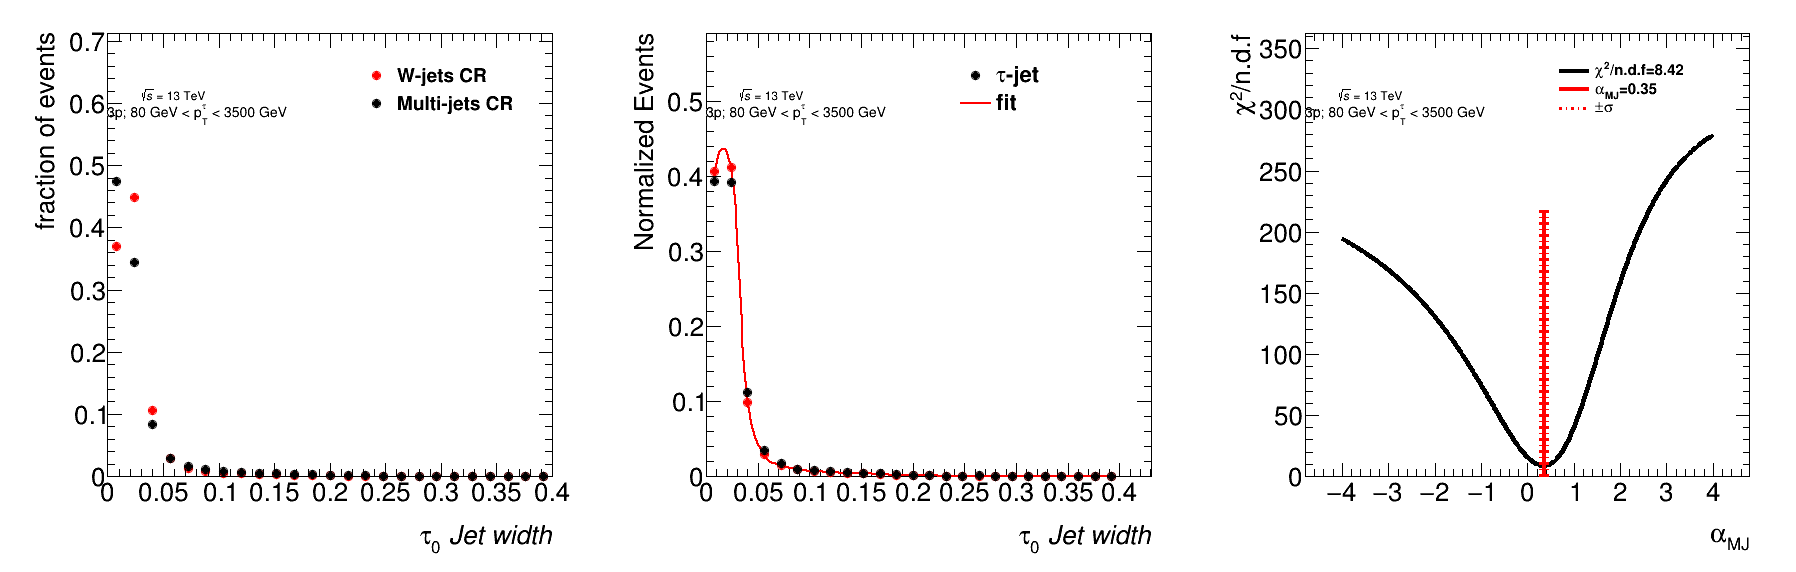
\includegraphics[width=1\textwidth]{chapters/chapter6_HPlus/images/FFs/FFs_FIT_SR_TAUJET_3_80_3500.png}

	\end{center}
	\caption{
	Estimation of $\alpha_\mathrm{MJ}$ in the \tauhad+jets signal region for
	3-prong \tauhad\ candidates. Left: templates of discriminating variables for different \tauhad\ $\pt$
	and n-prong slices. Middle: shape of the discriminating variable obtained in the signal region and fitted
	shape using the templates measured in the control regions. Right: $\chi^2/\mathrm{ndf}$ of the fit as a
	function of $\alpha_\mathrm{MJ}$, the error on $\alpha_\mathrm{MJ}$ is defined by the band at
	$\chi^2_\mathrm{min}/\mathrm{ndf}+\sqrt{\frac{2}{\mathrm{ndf}}}$.
	}
	\label{fig:mm:Fits:region3_3}
	\end{figure}

	\begin{figure}
	\begin{center}
	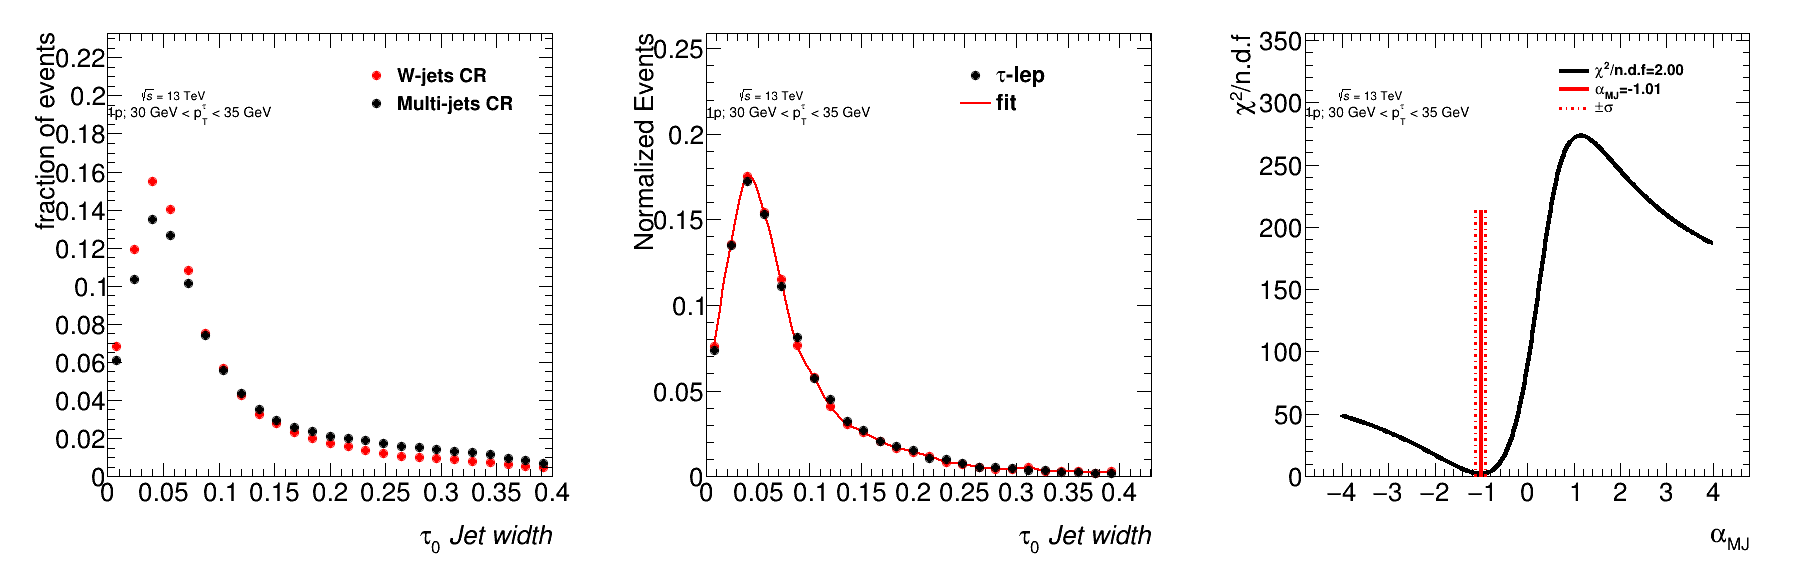
\includegraphics[width=1\textwidth]{chapters/chapter6_HPlus/images/FFs/FFs_FIT_SR_TAULEP_1_30_35.png}
	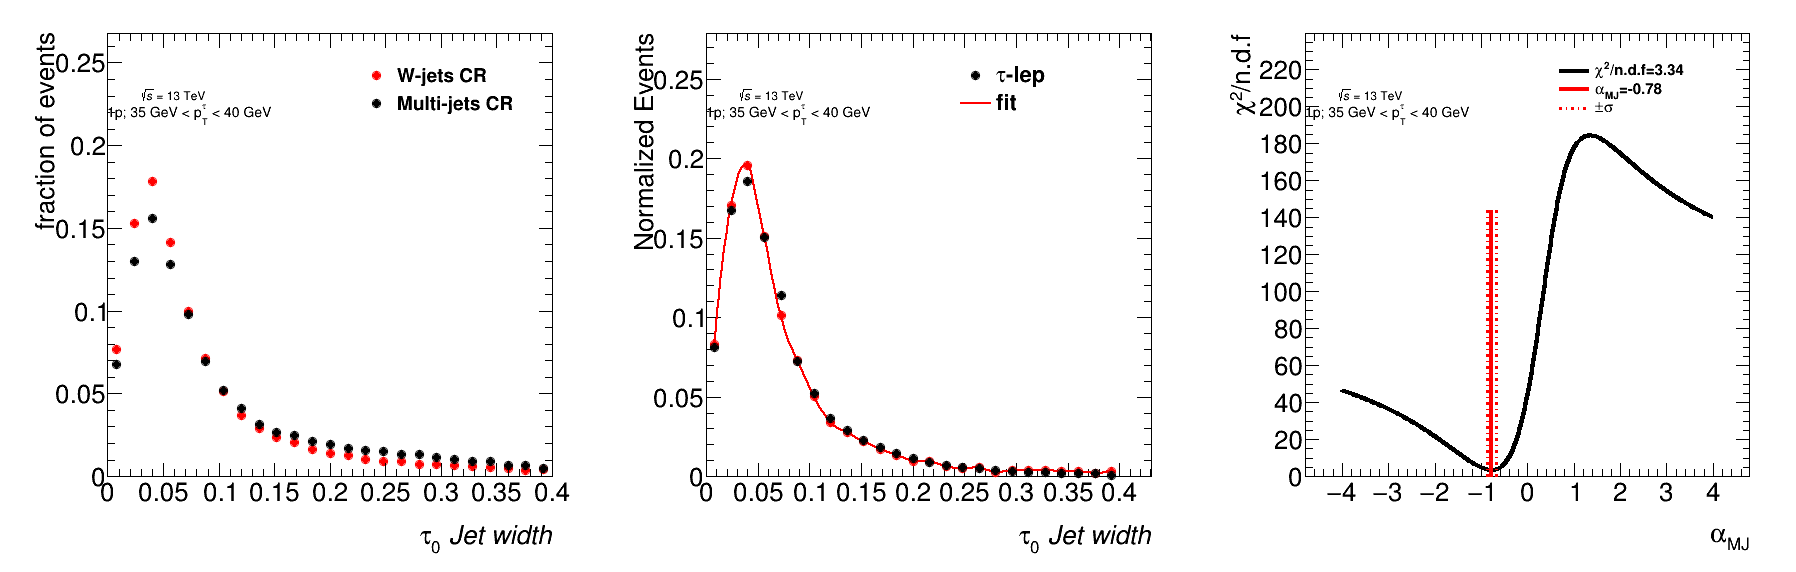
\includegraphics[width=1\textwidth]{chapters/chapter6_HPlus/images/FFs/FFs_FIT_SR_TAULEP_1_35_40.png}
	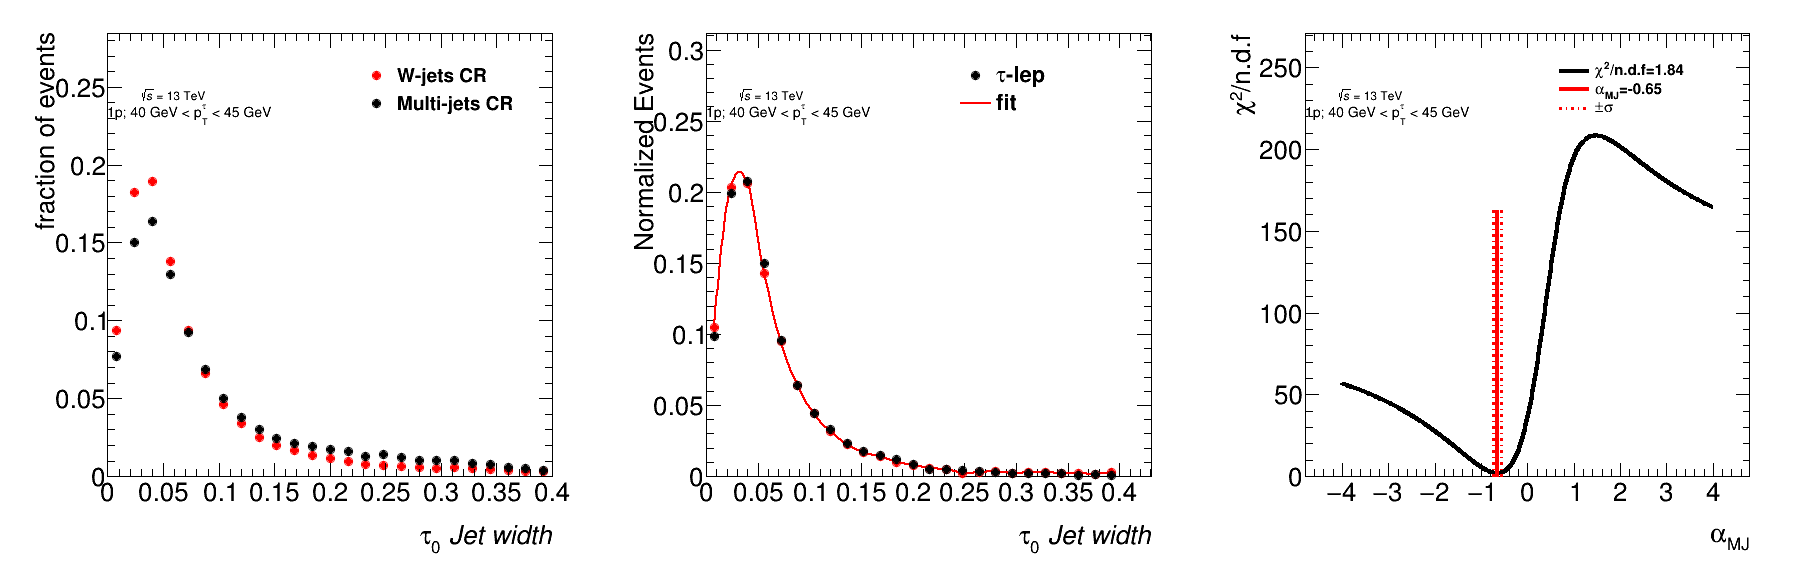
\includegraphics[width=1\textwidth]{chapters/chapter6_HPlus/images/FFs/FFs_FIT_SR_TAULEP_1_40_45.png}
	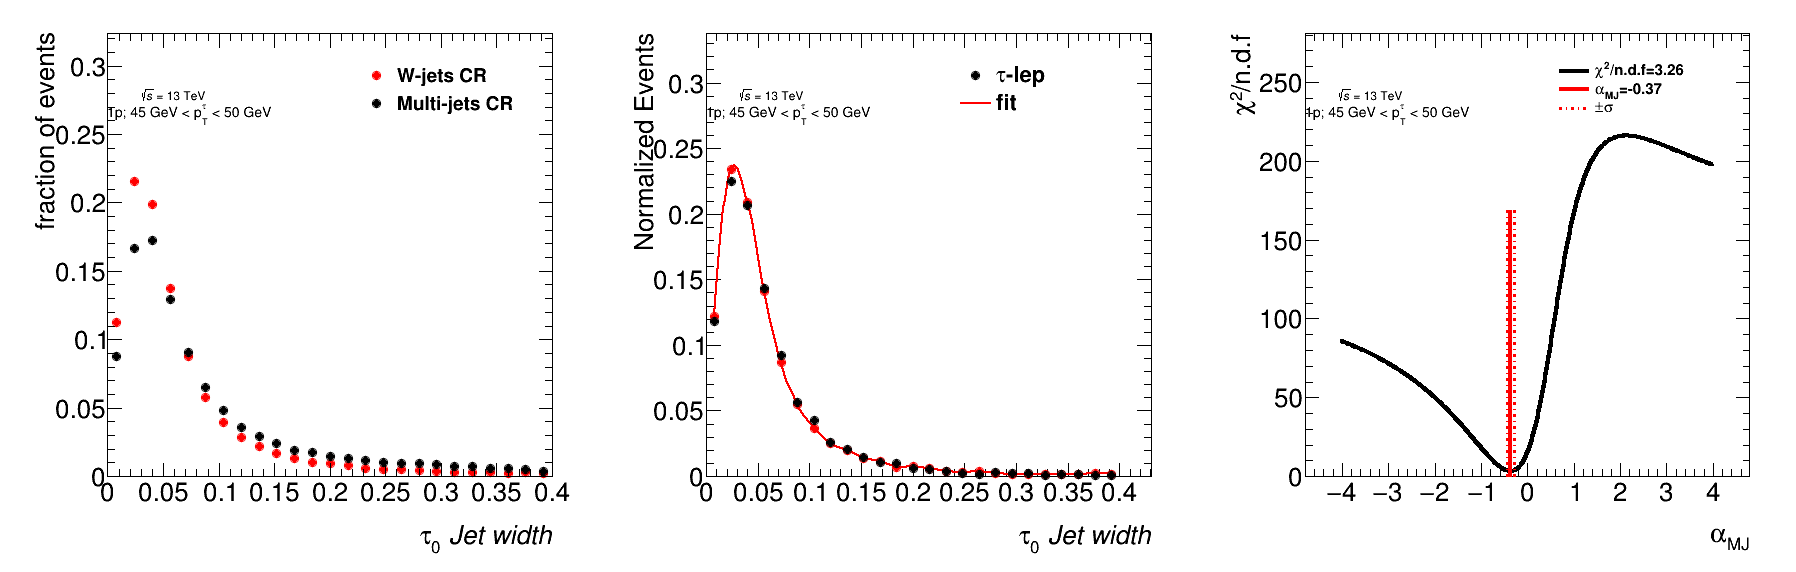
\includegraphics[width=1\textwidth]{chapters/chapter6_HPlus/images/FFs/FFs_FIT_SR_TAULEP_1_45_50.png}
	\end{center}
	\caption{
	Estimation of $\alpha_\mathrm{MJ}$ in the \tauhad+lepton signal region for $\pt \leq 50 GeV$
	1-prong \tauhad\ candidates. Left: templates of discriminating variables for different \tauhad\ $\pt$
	and n-prong slices. Middle: shape of the discriminating variable obtained in the signal region and fitted
	shape using the templates measured in the control regions. Right: $\chi^2/\mathrm{ndf}$ of the fit as a
	function of $\alpha_\mathrm{MJ}$, the error on $\alpha_\mathrm{MJ}$ is defined by the band at
	$\chi^2_\mathrm{min}/\mathrm{ndf}+\sqrt{\frac{2}{\mathrm{ndf}}}$.
	}
	\label{fig:mm:Fits:region7_1}
	\end{figure}


	\begin{figure}
	\begin{center}
	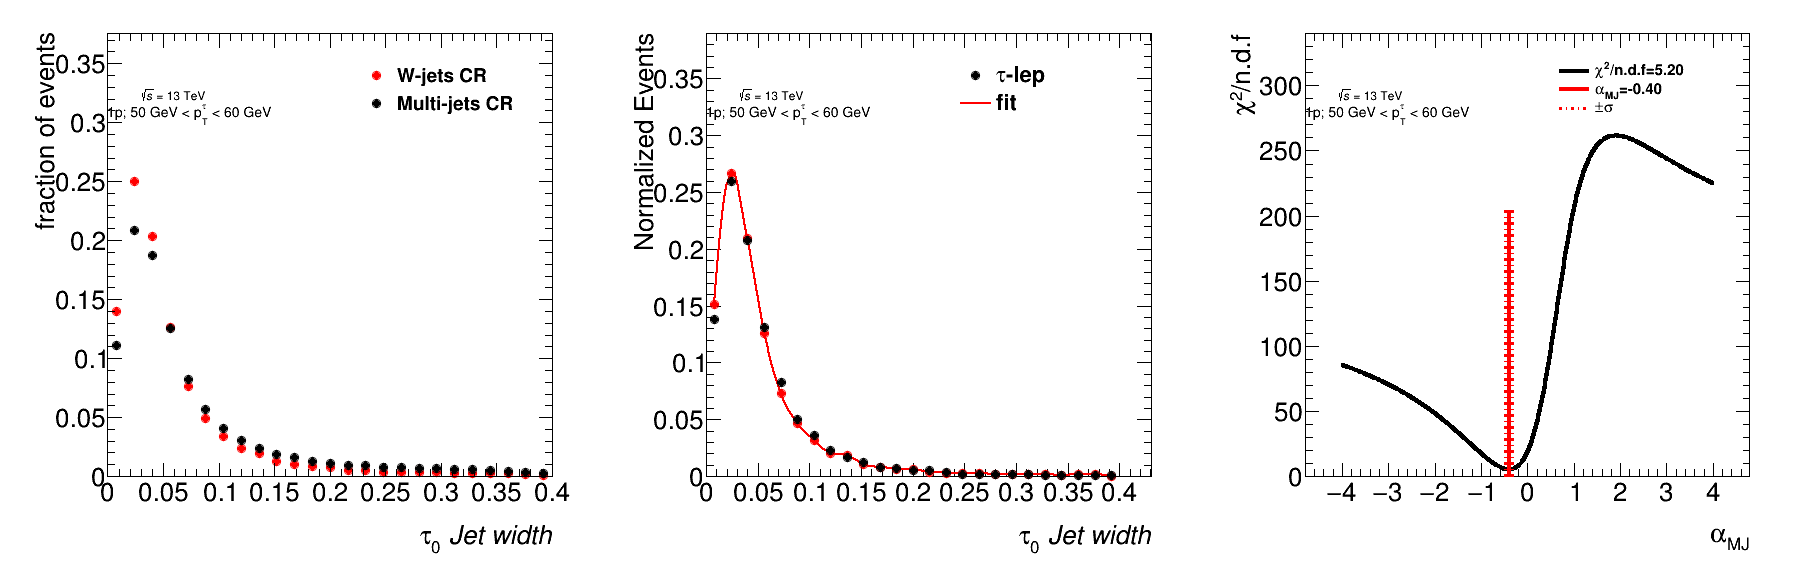
\includegraphics[width=1\textwidth]{chapters/chapter6_HPlus/images/FFs/FFs_FIT_SR_TAULEP_1_50_60.png}
	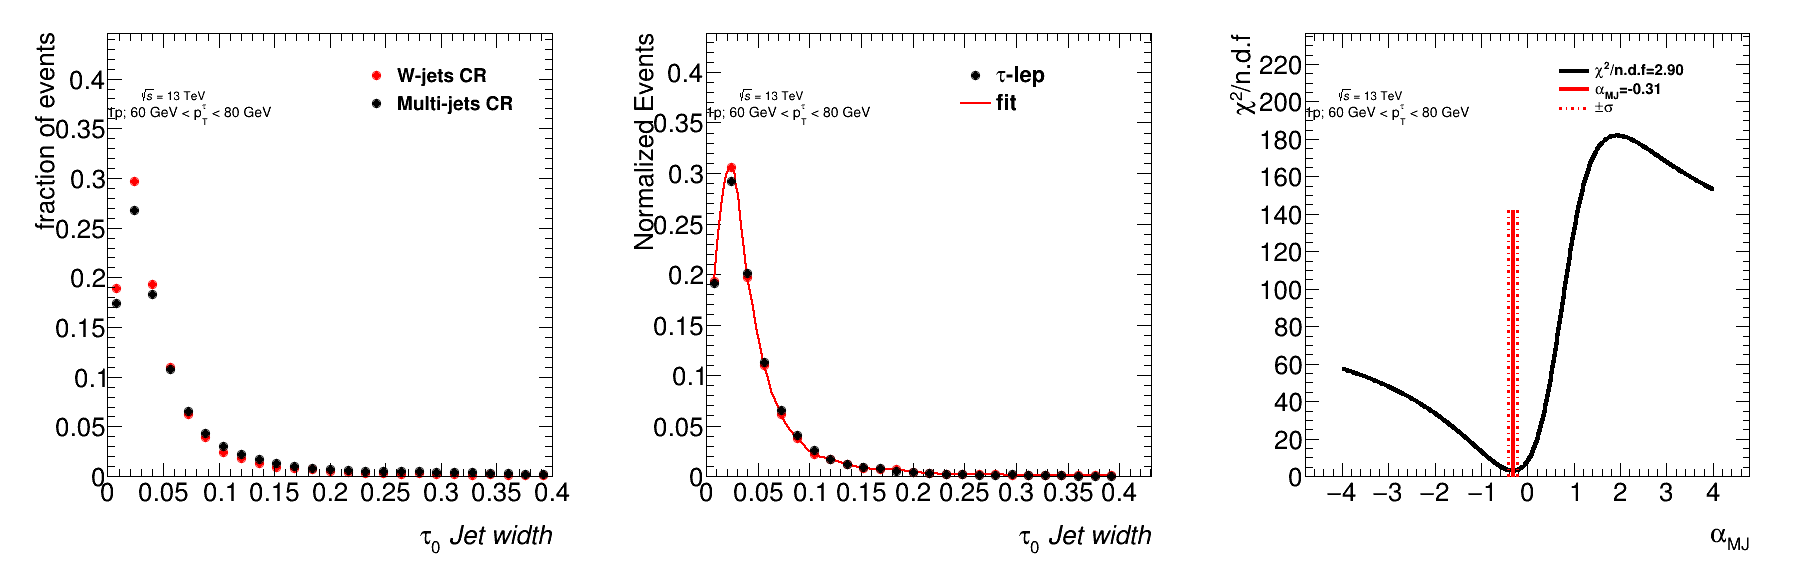
\includegraphics[width=1\textwidth]{chapters/chapter6_HPlus/images/FFs/FFs_FIT_SR_TAULEP_1_60_80.png}
	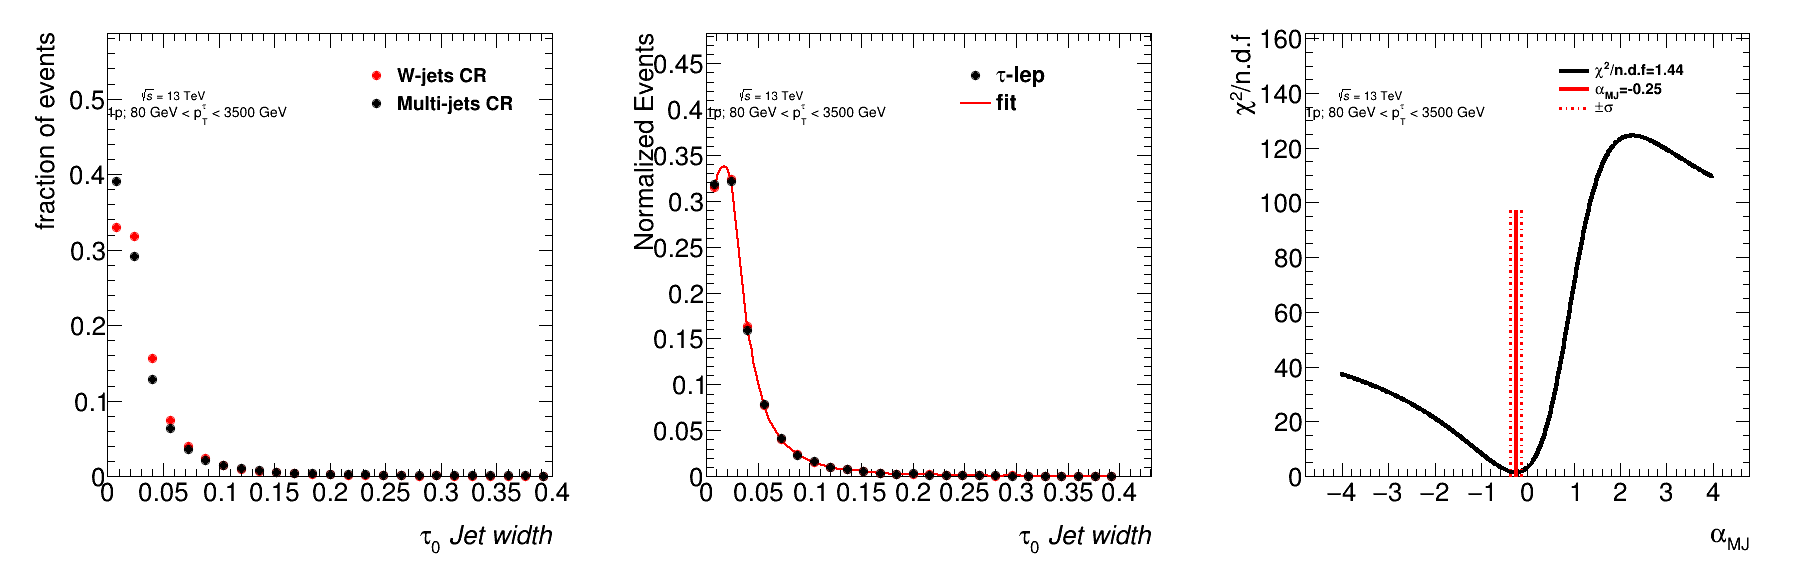
\includegraphics[width=1\textwidth]{chapters/chapter6_HPlus/images/FFs/FFs_FIT_SR_TAULEP_1_80_3500.png}
	\end{center}
	\caption{
	Estimation of $\alpha_\mathrm{MJ}$ in the \tauhad+lepton signal region for $\pt \geq 50 GeV$
	1-prong \tauhad\ candidates. Left: templates of discriminating variables for different \tauhad\ $\pt$
	and n-prong slices. Middle: shape of the discriminating variable obtained in the signal region and fitted
	shape using the templates measured in the control regions. Right: $\chi^2/\mathrm{ndf}$ of the fit as a
	function of $\alpha_\mathrm{MJ}$, the error on $\alpha_\mathrm{MJ}$ is defined by the band at
	$\chi^2_\mathrm{min}/\mathrm{ndf}+\sqrt{\frac{2}{\mathrm{ndf}}}$.
	}
	\label{fig:mm:Fits:region7_2}
	\end{figure}



	\begin{figure}
	\begin{center}
	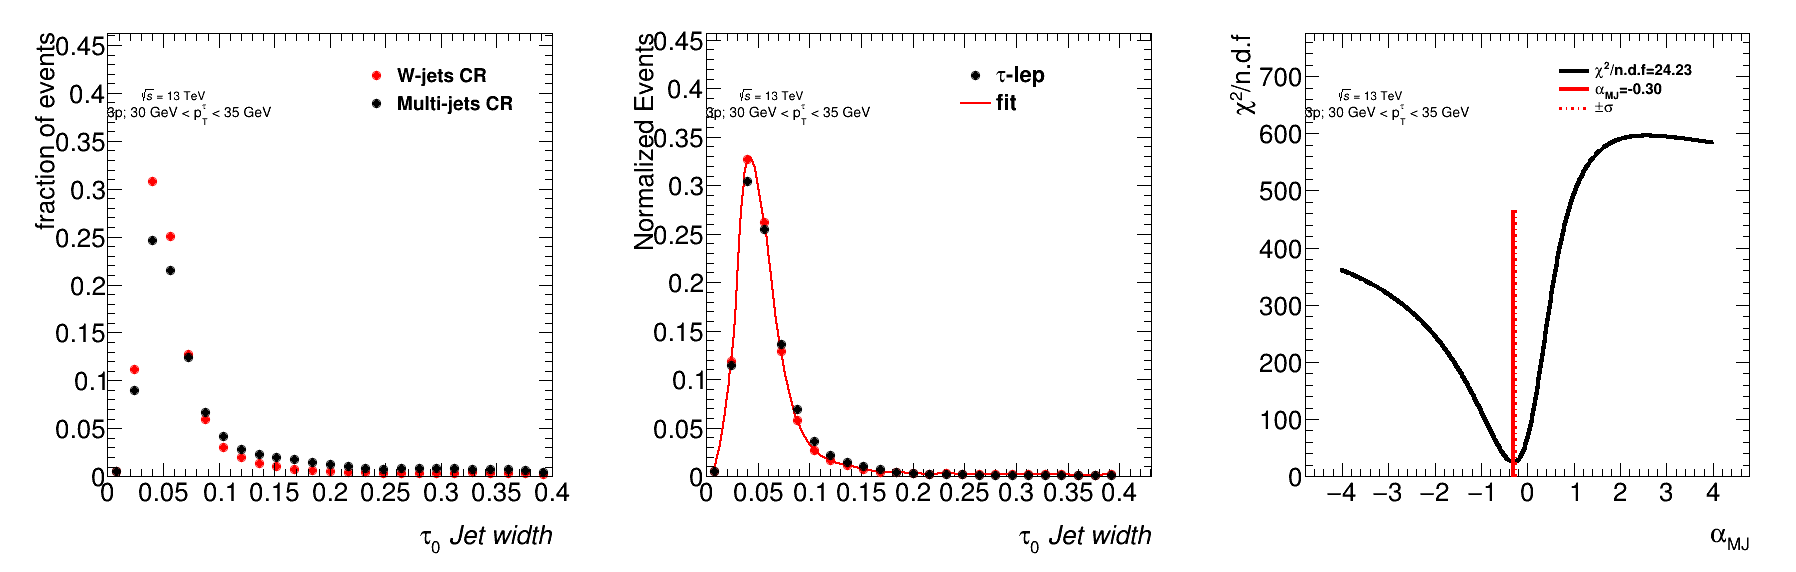
\includegraphics[width=1\textwidth]{chapters/chapter6_HPlus/images/FFs/FFs_FIT_SR_TAULEP_3_30_35.png}
	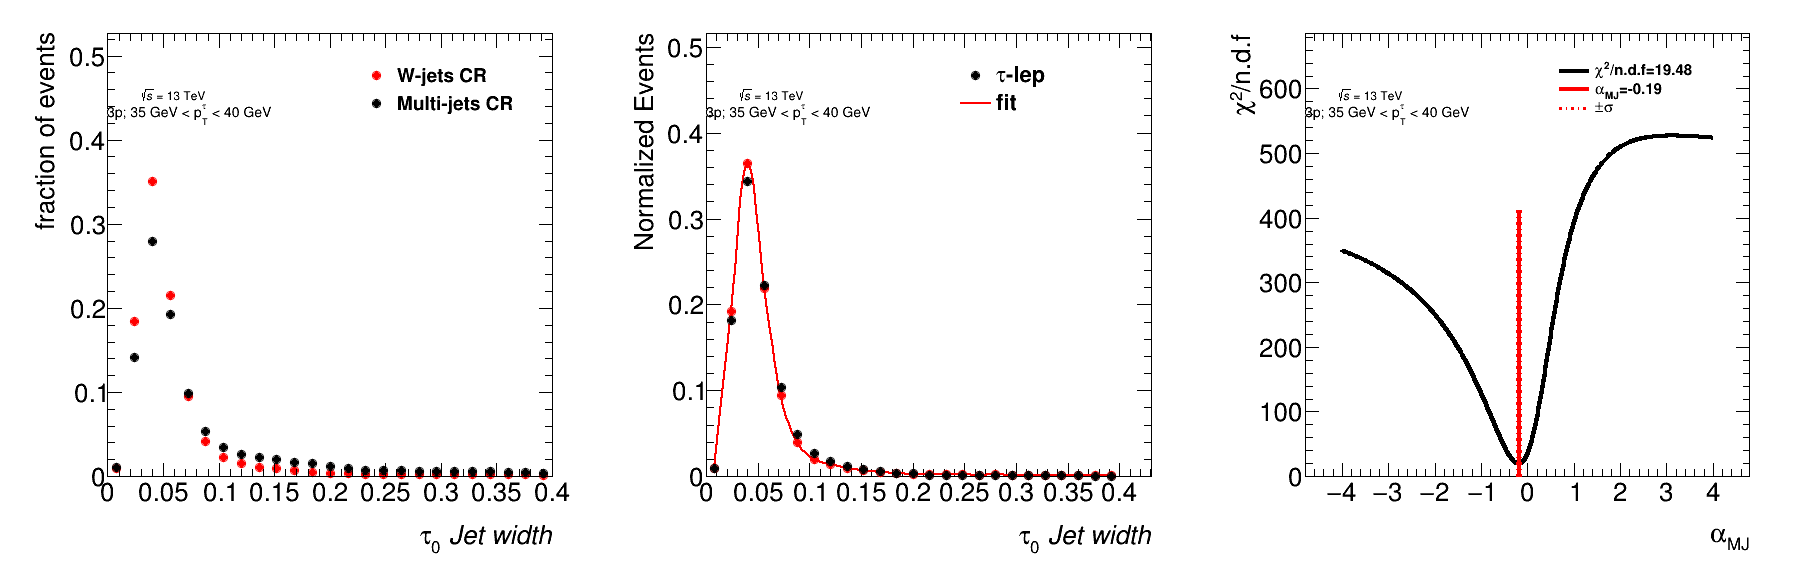
\includegraphics[width=1\textwidth]{chapters/chapter6_HPlus/images/FFs/FFs_FIT_SR_TAULEP_3_35_40.png}
	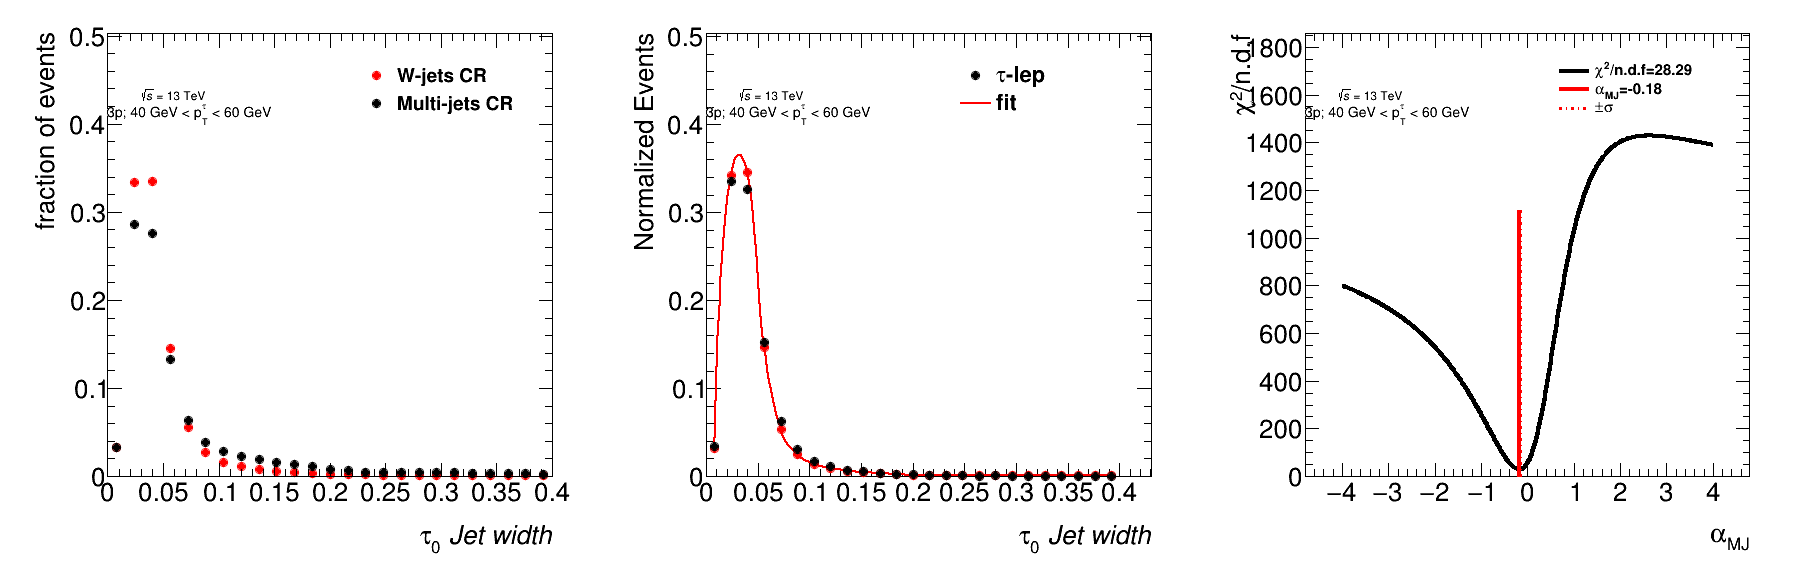
\includegraphics[width=1\textwidth]{chapters/chapter6_HPlus/images/FFs/FFs_FIT_SR_TAULEP_3_40_60.png}
	\end{center}
	\caption{
	Estimation of $\alpha_\mathrm{MJ}$ in the \tauhad+lepton signal region for $\pt \leq 60 GeV$
	3-prong \tauhad\ candidates. Left: templates of discriminating variables for different \tauhad\ $\pt$
	and n-prong slices. Middle: shape of the discriminating variable obtained in the signal region and fitted
	shape using the templates measured in the control regions. Right: $\chi^2/\mathrm{ndf}$ of the fit as a
	function of $\alpha_\mathrm{MJ}$, the error on $\alpha_\mathrm{MJ}$ is defined by the band at
	$\chi^2_\mathrm{min}/\mathrm{ndf}+\sqrt{\frac{2}{\mathrm{ndf}}}$.
	}
	\label{fig:mm:Fits:region7_3}
	\end{figure}

	\begin{figure}
	\begin{center}
	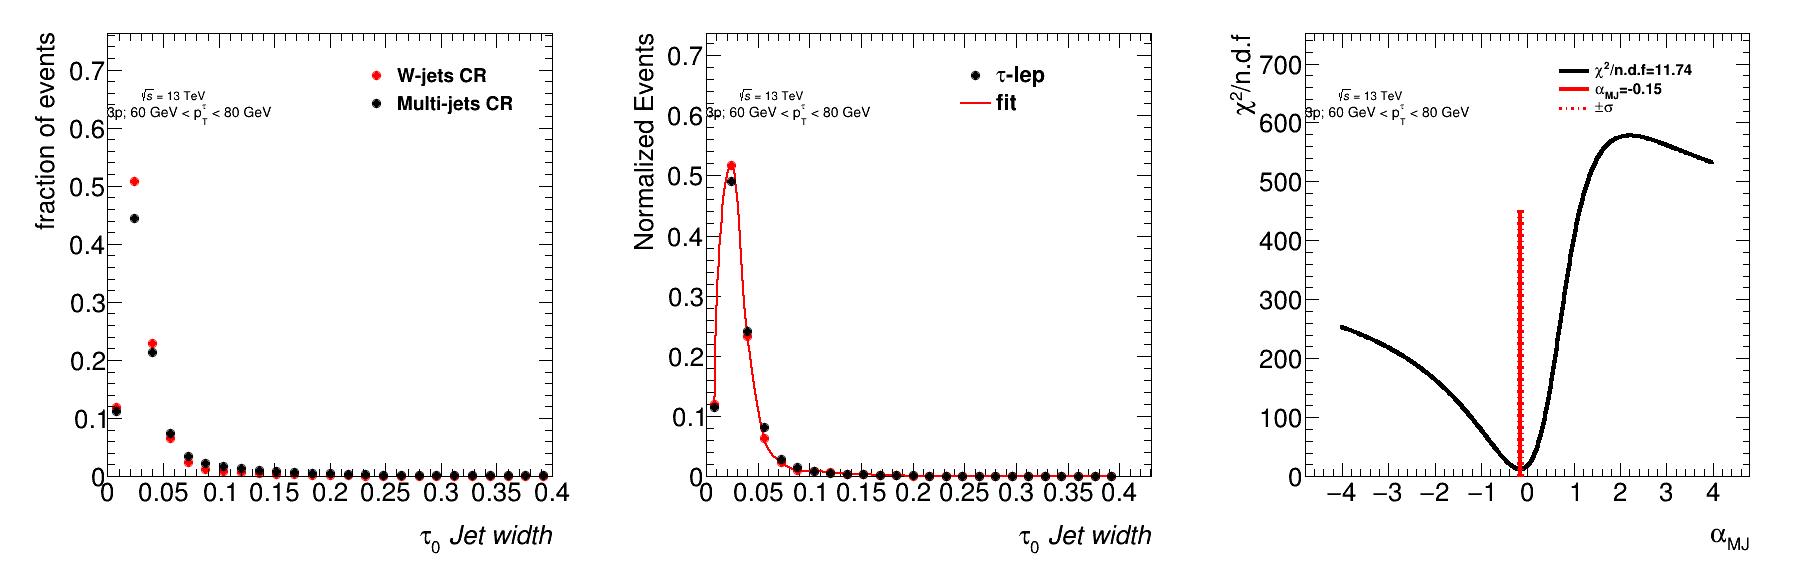
\includegraphics[width=1\textwidth]{chapters/chapter6_HPlus/images/FFs/FFs_FIT_SR_TAULEP_3_60_80.png}
	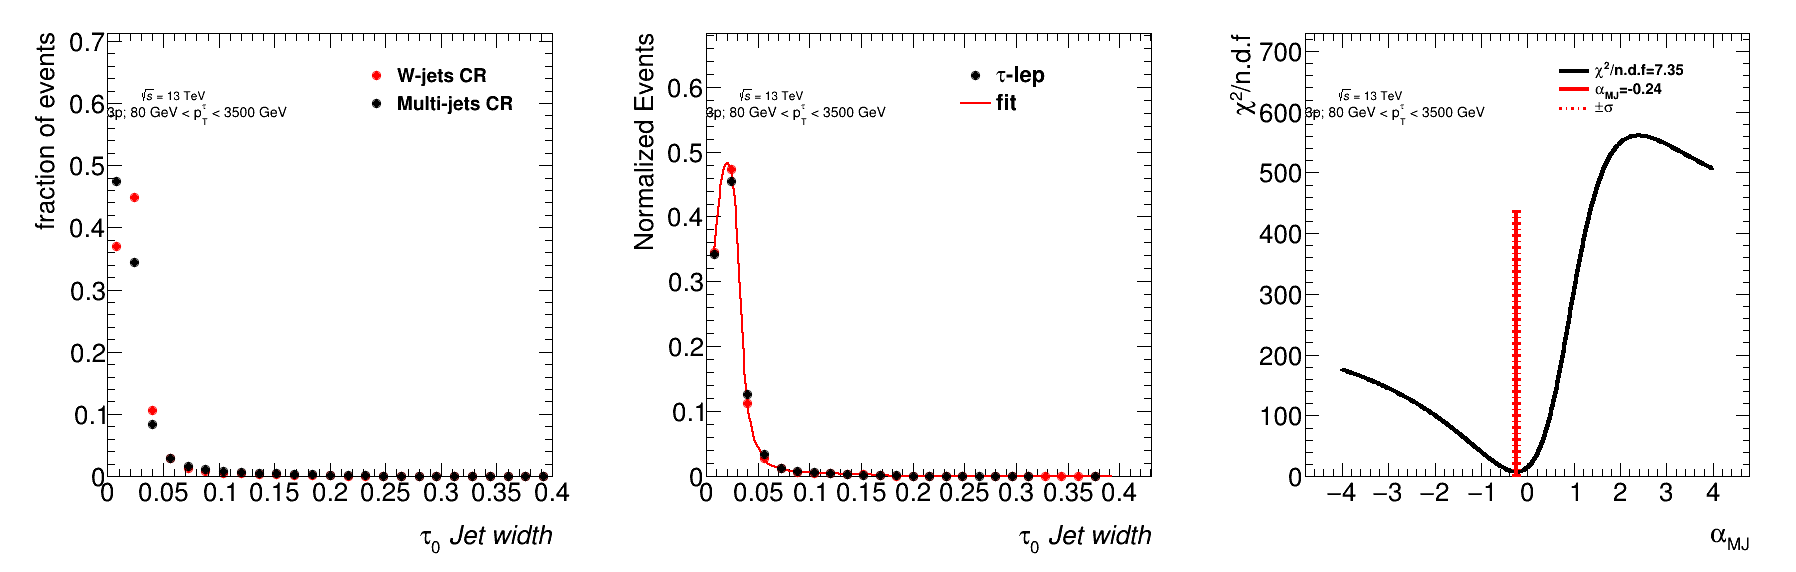
\includegraphics[width=1\textwidth]{chapters/chapter6_HPlus/images/FFs/FFs_FIT_SR_TAULEP_3_80_3500.png}
	\end{center}
	\caption{
	Estimation of $\alpha_\mathrm{MJ}$ in the \tauhad+lepton signal region for $\pt \geq 60 GeV$
	3-prong \tauhad\ candidates. Left: templates of discriminating variables for different \tauhad\ $\pt$
	and n-prong slices. Middle: shape of the discriminating variable obtained in the signal region and fitted
	shape using the templates measured in the control regions. Right: $\chi^2/\mathrm{ndf}$ of the fit as a
	function of $\alpha_\mathrm{MJ}$, the error on $\alpha_\mathrm{MJ}$ is defined by the band at
	$\chi^2_\mathrm{min}/\mathrm{ndf}+\sqrt{\frac{2}{\mathrm{ndf}}}$.
	}
	\label{fig:mm:Fits:region7_4}
	\end{figure}